% !TEX root = hw12-answers-graded.tex
\chead{\textbf{Exercises week 12}}
\begin{document}
\flushleft\textbf{Topic: Counterfactual bounds and causal discovery}

\begin{enumerate}
	\item %($2+2+1 ~(+ 2) + 1$ points) 
	Consider the coin machine in Figure \ref{fig:coin_machine}.

	\begin{figure}[H]
		\centering
		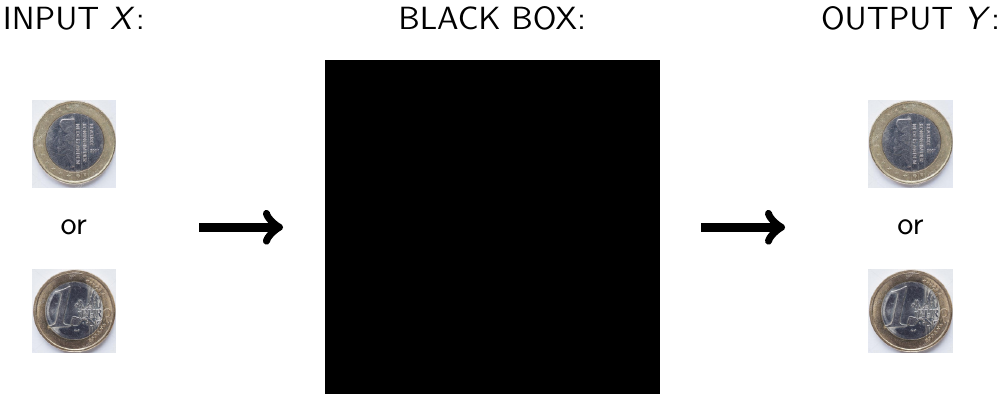
\includegraphics[width=0.8\textwidth]{blackbox}
		\caption{The mysterious coin machine}
		\label{fig:coin_machine}
	\end{figure}

	One can insert a coin with either heads or tails up (modeled as $X = +1$ and $X = -1$, respectively), and a few seconds later, it outputs the same coin, again with either heads or tails up (modeled as $Y = +1$ and $Y = -1$, respectively), i.e. the machine can flip the coin along the way.
	%Suppose you observe someone repeatedly inputting coins into the machine, which subsequently outputs each coin again with some orientation.
	%You gather data from this observational distribution $P(X, Y)$.
	You can conduct an experiment by inserting many coins into the machine and observing the outcomes. This leads you to collect data for the Markov kernel $P(Y | \text{do}(X))$.
	After collecting lots of data and estimating both distributions based on them, you obtain the following Markov kernel:
	\vspace{20pt}

	\centerline{\begin{tabular}{cc|c}
			$x$ & $y$ & $P(Y = y | \text{do}(X = x))$ \\
			\hline
			-1  & -1  & 1/2                           \\
			-1  & 1   & 1/2                           \\
			\hline
			1   & -1  & 1/2                           \\
			1   & 1   & 1/2                           \\
		\end{tabular}}
	\vspace{15pt}
	This seems like a rather boring machine.
	But, is it?

	\begin{enumerate}
		\item Formally define two different SCMs $M$ and $\tilde{M}$ that model the mysterious coin machine, such that their observational Markov kernels agree with the one in the table above, and prove this agreement. Thereby, consider $X$ as an exogenous input variable and $Y$ as an endogenous variable. Construct the two SCMs in such a way that they will turn out to not be counterfactually equivalent (which you will then prove in the second part).

		\emph{Hint: Think of two different causal mechanisms, one which ignores the input orientation, and another one which makes use of it.}

		\item Prove that your two models $M$ and $\tilde{M}$ are observationally and interventionally equivalent, but not counterfactually equivalent (with respect to $O = \{Y\}$).
		% \item Come up with a physical mechanism which could implement your causal models $M$ and $\tilde{M}$ in the real world.
	\end{enumerate}
	% We're aiming at computing a lower and upper bound on the counterfactual probability $P((Y')^{\doit(x'=1)}=1|Y^{\doit(x=-1)}=-1)$, similar to Example \ref*{ex:Bounding_counterfactuals}. We'll use the following claim that the SCM $M_\rho$ from the Example is 'canonical': for every SCM $M=\langle \{X\}, \{Y\}, \{W\}, \{-1,1\}^2\times \Xcal_W, P_W, f \rangle$, there is a parametrisation $\rho$ of the SCM $M_\rho$ from Example \ref*{ex:Bounding_counterfactuals} such that $M$ and $M_\rho$ are counterfactually equivalent.
	\begin{enumerate}[resume*]
		% \item \textbf{BONUS} Prove the above claim that for any SCM $M$ (with one binary input variable $X$ and one binary output variable $Y$) there is a counterfactually equivalent $M_\rho$.
		\item Derive, using Example \ref*{ex:Bounding_counterfactuals}, a lower and upper bound for $P((Y')^{\doit(x'=1)}=1|Y^{\doit(x=-1)}=-1)$.
		%  If you haven't done 1d, you may assume that the claim holds true.
		\item Similar to Example \ref*{ex:Bounding_counterfactuals}, consider a causal mechanism $Y^{\doit(x)} = f_W(x)$ with
		\begin{center}\begin{tabular}{c|rrrr}
				$x$ & $f_{-1,-1}(x)$ & $f_{-1,1}(x)$ & $f_{1,-1}(x)$ & $f_{1,1}(x)$ \\
				\hline
				-1  & -1             & -1            & 1             & 1            \\
				1   & -1             & 1             & -1            & 1
			\end{tabular}\end{center}
		with exogenous distribution $P(W=w) = \rho_w$, where $\rho_{-1,-1} = \rho_{-1,1} = \tfrac{\alpha}{2}$ and $\rho_{1-1}=\rho_{11}=\tfrac{1-\alpha}{2}$ for some $0 < \alpha < 1$.

		Check that we indeed have $P(Y^{\doit(x)} = y) = P(Y = y|\doit(X=x)) = \tfrac{1}{2}$ for all $x,y\in\{-1,1\}$. Then, derive a lower and upper bound for $P((Y')^{\doit(x'=1)}=1|Y^{\doit(x=-1)}=-1)$, for both where $\alpha < 1/2$ and $\alpha > 1/2$. What happens when $\alpha$ approaches 1?
	\end{enumerate}


	\begin{ungradedsolution}
		\begin{enumerate}
			\item We define $M = \left\langle X, Y, W, \{-1,1\}^3, \text{Bernoulli}(1/2), f \right\rangle$ with
			\begin{equation*}
				f: \{-1,1\}^3 \to \{-1,1\}, \quad f(x, y, w) := w,
			\end{equation*}
			which simply outputs the coin in random orientation, independent of the input orientation.

			In contrast, we define $\tilde{M} = \left\langle X, Y, W, \{-1,1\}^3, \text{Bernoulli}(1/2), \tilde{f} \right\rangle$, with the causal mechanism given by
			\begin{equation*}
				\tilde{f}: \{-1,1\}^3 \to \{-1,1\}, \quad \tilde{f}(x, y, w) = x \cdot w,
			\end{equation*}
			which randomly decides whether to \emph{flip} the input orientation, and thus creates an output which depends functionally on the input.

			In order to show that the Markov kernels agree with the table, we first need the solution functions.
			As can easily be checked, the unique solution functions are given by
			\begin{align*}
				g: \{-1,1\}^2 \to \{-1,1\},        & \quad g(x, w) = w          \\
				\tilde{g}: \{-1,1\}^2 \to \{-1,1\} & \quad g(x, w) = x \cdot w.
			\end{align*}
			Since they are unique, they define unique observational Markov kernels by Theorem 8.1.2, where we abbreviate the Bernoulli(1/2) distribution with $P$:
			\begin{align*}
				g_{*}P(W | X): \mathcal{X}_X \dashrightarrow \mathcal{X}_Y, \quad (y | x)         & \mapsto P\big(g^{-1}(y)_x\big) = P\big(\{w | w = g(w,x) = y\}\big) = \frac{1}{2}                                                      \\
				\tilde{g}_{*}P(W | X): \mathcal{X}_X \dashrightarrow \mathcal{X}_Y, \quad (y | x) & \mapsto P\left(\tilde{g}^{-1}(y)_x\right) = P\left(\{w | x \cdot w = \tilde{g}(w, x) = y \}\right) = P\left(y/x\right) = \frac{1}{2}.
			\end{align*}
			Note that by definition, we have $P_{M}(Y | \text{do}(X)) = g_{*}P(W | X)$, and $P_{\tilde{M}}(Y | \text{do}(X)) = \tilde{g}_{*}P(W | X)$.
			Thus, we have proven $P_{M}(Y = y | \text{do}(X = x)) = 1/2$ and $P_{\tilde{M}}(Y = y | \text{do}(X = x)) = 1/2$ for all combinations of $x$ and $y$.
			This shows that the observational Markov kernels of our causal models agree with the table.
			\item Observational equivalence is precisely the statement that the observational Markov kernels agree, which holds since they both agree with the table.

			For interventional equivalence, note that we only need to show two observational equivalences:
			That $M_{\text{do}(\emptyset)}$ is observationally equivalent to $\tilde{M}_{\text{do}(\emptyset)}$ holds since intervention with the emptyset does not change the causal models.
			That $M_{\text{do}(Y)}$ is observationally equivalent to $\tilde{M}_{\text{do}(Y)}$ holds trivially since $M$ and $\tilde{M}$ differ only in their causal mechanism, and this is removed completely by making $Y$ an exogenous variable.

			Thus, we are only left with proving that these models are \emph{not} counterfactually equivalent.
			For this, we explicitly construct the twinned SCMs:
			\begin{align*}
				M^{\text{twin}} = \left\langle \{X, X'\}, \{Y, Y'\}, W, \{-1,1\}^5, f \times f' \right\rangle, \ \ \text{with} \\
				(f\times f')(x, x', y, y', w)  = (w, w) \in \{-1,1\}^2
			\end{align*}
			And:
			\begin{align*}
				\tilde{M}^{\text{twin}} = \left\langle \{X, X'\}, \{Y, Y'\}, W, \{-1,1\}^5, \tilde{f} \times \tilde{f}' \right\rangle, \ \ \text{with} \\
				(\tilde{f} \times \tilde{f}')(x, x', y, y', w) = (x \cdot w, x' \cdot w) \in \{-1, 1\}^2.
			\end{align*}
			By definition, we need to show that they are not interventionally equivalent.
			Since interventional equivalence includes observational equivalence, it is enough to show that they are not even observationally equivalent.
			Thus, let's construct their observational Markov kernels.
			The (obviously unique) solution functions are given by
			\begin{align*}
				g^{\text{twin}}: \{-1,1\}^3 \to \{-1,1\}^2,         & \quad (x, x', w) \mapsto (w, w)                   \\
				\tilde{g}^{\text{twin}}: \{-1,1\}^3 \to \{-1,1\}^2, & \quad (x, x', w) \mapsto (x \cdot w, x' \cdot w).
			\end{align*}
			From this, we can construct the observational Markov kernels:
			\begin{align*}
				g^{\text{twin}}_* P(W | X, X'): \ \  & \mathcal{X}_{\{X,X'\}} \dashrightarrow \mathcal{X}_{\{Y,Y'\}}            \\
				(y, y' | x, x')                      & \mapsto P\left((g^{\text{twin}})^{-1}(y, y')_{(x,x')}\right)             \\
				                                     & = P\left(\{w | (w,w) = g^{\text{twin}}(x, x', w) = (y, y')\right)        \\
				                                     & = \begin{cases} 0, \ \ \ y \neq y' \\ 1/2, \ \ \ \text{else}.\end{cases}
			\end{align*}
			And:
			\begin{align*}
				\tilde{g}^{\text{twin}}_* P(W | X, X'): \ \  & \mathcal{X}_{\{X,X'\}} \dashrightarrow \mathcal{X}_{Y,Y'\}}                                   \\
				(y, y' | x, x')                              & \mapsto P\left((\tilde{g}_{\text{twin}})^{-1}(y,y')_{(x,x')}\right)                           \\
				                                             & = P\left(\{w | (x \cdot w, x' \cdot w) = \tilde{g}^{\text{twin}}(x, x', w) = (y, y')\}\right) \\
				                                             & = P\left(\{w | y/x = w = y'/x'\right)                                                         \\
				                                             & = \begin{cases} 0, \ \ \ y/x \neq y'/x' \\ 1/2, \ \ \ \text{else}.\end{cases}
			\end{align*}
			These are simply not the same Markov kernels, which can be seen for example in the case $y = y'$ and $x \neq x'$, which proves the claim that they are not counterfactually equivalent.

			\textbf{Addendum:} To get some more intuitions, we now express the difference of the Markov kernels using counterfactual distributions.
			For this, set
			\begin{align*}
				P_{M}(Y, Y' | \text{do}(X), \text{do}(X'))         & := g_{*}^{\text{twin}}P(W | X, X'), \text{ and } \\
				P_{\tilde{M}}(Y, Y' | \text{do}(X), \text{do}(X')) & :=  \tilde{g}_*^{\text{twin}}P(W | X, X').
			\end{align*}
			Counterfactual distributions are then expressed by conditioning the Markov kernels on $Y$, i.e. on the ``original outcome''.
			In the case $y = y'$ and $x \neq x'$, we then obtain:
			\begin{align*}
				P_{M}(Y' = y' | Y = y, \doit(X = x), \doit(X' = x')) & = \frac{P_{M}(Y' = y', Y = y | \doit(X = x), \doit(X' = x'))}{P_{M}(Y = y | \doit(X = x) \doit(X ' = x'))} \\
				                                                     & = \frac{1/2}{P_{M}(Y = y | \doit(X = x))}                                                                  \\
				                                                     & = \frac{1/2}{1/2}                                                                                          \\
				                                                     & = 1.
			\end{align*}
			In the second step, we have used that the marginal Markov kernel in which $Y'$ is ``marginalized out'' does not depend on $X'$ anymore, as can easily be shown in general such situations.
			Similarly, one can show that $P_{\tilde{M}}(Y' = y' | Y = y, \doit(X = X), \doit(X' = x')) = 0$.
			Thus, the counterfactual distributions are different.

			This is the expected outcome: The first model does not care about the input at all, and so if the ``randomness'' $w$ is the same in the actual, and the counterfactual world, then the outcome $y = y'$ is the same.
			However, the second model multiplies the ``randomness'' $w$ with the input $x$ or $x'$, and so if the input changes, the output also must change, and so we cannot have the outcome $y' = y$.

			% \item $M$ could be implemented physically by tossing a second coin internally, and then orienting the coin which was input in accordance to the internal coin toss.
			% $\tilde{M}$ can be implemented by tossing a second coin internally, and then flipping the coin which was input based on the result of the internal coin toss.
			% Assuming that the internal coin toss happens each time already before the coin is put in, this means that it is already pre-determined whether the coin will come out heads or tails (implementation 1) or whether it will be flipped along the way (second model), meaning that the twinned SCM models counterfactuals correctly.

			% \item \textbf{Draft, we still have to prove counterfactual equivalence:} For a given SCM $M = \langle\{X\}, \{Y\}, \{W\}, \{0,1\}^2\times \Xcal_W, P_W, f\rangle$, we can define the random variable $\hat{W}$ taking values in $\{0,1\}$, and with distribution $\rho_{yy'} := P(\hat{W} = (y,y')) := P(Y^{\doit(X=0)}=y, (Y')^{\doit(X'=1)})$, where this latter probability corresponds to the observational distribution of $M^\twin$. Then, the SCM $M_\rho = \langle\{X\}, \{Y\}, \{\hat{W}\}, \{0,1\}^3, P_{\hat{W}}, \hat{f}\rangle$ with structural equation $\hat{f}(x, \hat{w}) := \hat{f}_{\hat{w}}(f)$, and
			% \begin{align*}
			% 	\hat{f}_{00} & : 0 \mapsto 0, 1\mapsto 0 \\
			% 	\hat{f}_{01} & : 0 \mapsto 0, 1\mapsto 1 \\
			% 	\hat{f}_{10} & : 0 \mapsto 1, 1\mapsto 0 \\
			% 	\hat{f}_{11} & : 0 \mapsto 1, 1\mapsto 1
			% \end{align*}
			% is indeed counterfactually equivalent to $M$: \textbf{TODO}.
			\item We have $p_{y|x}=1/2$ for all $x, y\in\{-1,1\}$ so from Example \ref*{ex:Bounding_counterfactuals} we immediately derive the trivial bound $0 \leq P((Y')^{\doit(x'=1)}=1|Y^{\doit(x=-1)}=-1) \leq 1$.
			\item Writing $p_{y|x} := P(Y^{\doit(x)})$ we have the following conditional probabilities:
			\begin{center}\begin{tabular}{rrr}
					$x$ & $y$ & $p_{y|x}$  \\
					\hline
					-1  & -1  & $\alpha$   \\ % = 1-eps
					-1  & 1   & $1-\alpha$ \\ %= eps
					1   & -1  & $1/2$      \\ %= delta
					1   & 1   & $1/2$      \\ %= 1-delta
				\end{tabular}\end{center}
			We can directly read off the bounds from Example \ref*{ex:Bounding_counterfactuals}. For $\alpha < 1/2$ we have $\min(p_{-1|-1}, p_{1|1}) = \alpha$, so
			$$0 \le P((Y')^{\doit(x=1)} = 1 | Y^{\doit(x=-1)}=-1) \le 1.$$
			For $\alpha > 1/2$ we have $\min(p_{-1|-1}, p_{1|1}) = 1/2$ so
			$$1 - \frac{1}{2\alpha} \le P((Y')^{\doit(x=1)} = 1 | Y^{\doit(x=-1)}=-1) \le \frac{1}{2\alpha}.$$
			Interestingly, letting $\alpha \to 1$ forces $P((Y')^{\doit(x=1)} | Y^{\doit(x=-1)}=-1)$ to a uniform distribution on $\{-1,1\}$.
		\end{enumerate}
	\end{ungradedsolution}
	% TODO 23/24: actually, here we can point-identify the quantity of interest, it is equal to 1/2, so it's uniform for any value of alpha

	\item 
	% TODO 23/24: the current proposition 8.3.2 does not prove counterfactual equivalence of this SCM... Also, students should elaborate on the parametrization: what is the function $f_U$ for particular values of $U$?
	% Also, they parametrised P(X=x, Y=y, U=u) = \rho_{xyu}, which doesn't allow for calculating counterfactual probabilities... Or does it? Check Jesus Abel Garcia his hw.
	% Add to the question: counterfactually equivalent wrt V.
	For bounding counterfactual probabilities, one needs to assume no confounding between cause and effect (as we are doing implicitly when bounding $P(Y | \doit(X, X'), Y)$).
	We will show that if we allow for latent confounding between $X$ and $Y$, we cannot find informative bounds for the quantity
	$$P_{M_{\rho}^{\twin}}((Y')^{\doit(x'=1)}=1\mid Y=0,X=0)$$
	\begin{enumerate}
		\item Consider an SCM $M=\langle J=\emptyset, V = \{X, Y\}, W=\{U\}, \{0,1\}^3, \textrm{Bernoulli}(p_u), f\rangle$ with some $p_u \in [0,1]$ and structural equations
		$$f(X, Y, U) = \begin{pmatrix}
				f_X(U)   \\
				f_Y(X,U) \\
			\end{pmatrix}$$ for some $f_X, f_Y$. Provide a counterfactually equivalent SCM $M_\rho$ with response function (structural equation) $f_U$, and response variable $U \in \{0,1\}^3$ with distribution $P(U)$ parametrized by $\rho \in \Delta_7$.
		\item Give the following distributions in terms of the parameters $\rho$:
		\begin{center}\begin{tabular}{ccll}
				$x$ & $y$ & $P(X=x, Y=y)$ & $P(Y=y\mid \doit(X=x))$ \\
				\hline
				0   & 0   &               &                         \\
				0   & 1   &               &                         \\
				1   & 0   &               &                         \\
				1   & 1   &               &
			\end{tabular}\end{center}
		\item Derive the distribution $P_{M_{\rho}^{\twin}}(U \mid X=0,Y=0)$ in terms of $\rho$.
		\item Derive the quantity $P_{M_{\rho}^{\twin}}((Y')^{\doit(x'=1)}=1\mid Y=0,X=0)$ in terms of $\rho$.
		\item Conclude that for any observed probabilities $p_{x,y} = P(X=x, Y=y)$ we can pick parameters $\rho$ that fit these observations, but that can let the quantity $P_{M_{\rho}^{\twin}}((Y')^{\doit(x'=1)}=1\mid Y=0,X=0)$ take any value in $(0,1)$. Hence there cannot exist informative bounds of this quantity.
	\end{enumerate}

	\begin{gradedsolution}
		\begin{enumerate}
			\item \points{1} We formulate the SCM $M=\langle J=\emptyset, V=\{X, Y\}, W=\{U\}, \{0,1\}^5, P(U), \tilde{f} \rangle$
			where $U \in \{0,1\}^3$, $U_1$ encodes the value of $X$, $U_2$ encodes the value of $Y$ if $X=0$ and $U_3$ encodes the value of $Y$ when $X=1$. Hence, the structural equation is
			$$\tilde{f}(X, Y, U) = \tilde{f}_U(X, Y) = \begin{pmatrix}
				U_1 \\
				U_2\cdot(1-X) + U_3\cdot X
			\end{pmatrix}$$
			and $P(U=(u_1,u_2,u_3)) = \rho_{u_1u_2u_3}$.
			\item \points{1}
			\begin{center}
				\begin{tabular}{ccll}
					$x$ & $y$ & $P(X=x, Y=y)$                   & $P(Y=y\mid\doit(X=x))$                                      \\
					\hline
					0   & 0   & $\rho_{000} + \rho_{001}$ & $\rho_{000} + \rho_{100} + \rho_{001} + \rho_{101}$ \\
					0   & 1   & $\rho_{010} + \rho_{011}$ & $\rho_{010} + \rho_{110} + \rho_{011} + \rho_{111}$ \\
					1   & 0   & $\rho_{100} + \rho_{110}$ & $\rho_{000} + \rho_{100} + \rho_{010} + \rho_{110}$ \\
					1   & 1   & $\rho_{101} + \rho_{111}$ & $\rho_{001} + \rho_{101} + \rho_{011} + \rho_{111}$
				\end{tabular}
			\end{center}
			\item \points{1} $$P_{M_{\rho}^{\twin}}(U \mid X=0,Y=0) = \frac{\rho_{000}}{\rho_{000} + \rho_{001}} \delta_{000} + \frac{\rho_{001}}{\rho_{000} + \rho_{001}} \delta_{001}$$
			\item \points{1} $$P_{M_{\rho}^{\twin}}((Y')^{\doit(x'=1)}=1\mid Y=0,X=0) = \frac{\rho_{001}}{\rho_{000} + \rho_{001}}$$
			\item \points{1} E.g.\ if we observe $P(X=0,Y=0) = \rho_{000} + \rho_{001} = p_1$ then we can pick parameters $\rho_{000}, \rho_{001}$ such that their sum equals the observed/estimated probability, and the counterfactual quantity $P_{M_{\rho}^{\twin}}((Y')^{\doit(x'=1)}=1\mid Y=0,X=0)$ can be made arbitrarily small or large in $(0,1)$.
		\end{enumerate}
	\end{gradedsolution}

	\item %(1 point) 
	Reichenbach's Principle of Common Cause states that if two events are dependent,
	then one must cause the other or the events are confounded (or any combination of these three possibilities).
	We can make this precise for simple SCMs in the following way. Assume that $M$
	is a simple SCM with two observed endogenous variables $X,Y$ (and possibly other
	latent variables as well, but no exogenous input nodes). Prove that
	$X \nIndep_{P_{M}} Y$
	implies that $X \to Y$,
	$X \leftarrow Y$ or $X \leftrightarrow Y$ in $G^{\{X,Y\}}(M)$.

	\begin{ungradedsolution}
		Assume that $X \to Y$, $X \leftarrow Y$ and $X \leftrightarrow Y$ \textbf{not} in $G^{\{X,Y\}}(M)$. Then $X$ is $\sigma$-separated from $Y$, and thus by Markov property $X \Indep_{P_{M}} Y$, which is a contradiction.
	\end{ungradedsolution}
\end{enumerate}
\end{document}
